\chapter{Systemintegration, Test und Validierung}
\label{cha:validierung}

In der finalen Phase des Wasserfall-Modells wird das integrierte Gesamtsystem validiert. Ziel dieser Phase ist es nachzuweisen, dass die in der Konzeptionsphase definierten Systemanforderungen (Requirements) durch die entwickelte Hard- und Software vollständig und fehlerfrei erfüllt werden.

\section{Testspezifikation (Test Cases)}
Um eine systematische Überprüfung zu gewährleisten, wurden die Kernanforderungen in konkrete Testfälle (Test Cases) überführt:
\begin{itemize}
	\item \textbf{TC1 -- Funktionale Kühlung (vgl. ID-0001, ID-0008):} Überprüfung, ob das System in der Lage ist, die Wassertemperatur kontinuierlich zu erfassen und die Flüssigkeit im Behälter durch die Aktorik herunterzukühlen.
	\item \textbf{TC2 -- User Interface \& Steuerung (vgl. ID-0010):} Verifizierung der verzögerungsfreien Reaktion des Systems auf Tastendrücke (Start/Stopp) sowie die korrekte Visualisierung der Zustände auf dem OLED-Display.
	\item \textbf{TC3 -- Systemstabilität \& Logging:} Test der seriellen Datenschnittstelle über einen längeren Zeitraum. Das eigens entwickelte Python-Skript muss die zyklischen Daten und Interrupt-Marker lückenlos empfangen, parsen und grafisch darstellen.
\end{itemize}

\section{Integrationstests}
Eine charakteristische Herausforderung des klassischen Wasserfall-Modells ist die späte Zusammenführung von Hardware und Software (Systemintegration). Erst in dieser Phase konnte das reale Zusammenspiel der elektronischen und programmiertechnischen Komponenten getestet werden. 

Bei der Integration von Aktorik und Sensorik zeigte sich, dass die gewählte Systemarchitektur grundsätzlich äußerst robust ist. Die getrennten Spannungsdomänen (12\,V für Aktorik, 3,3\,V für die Logik) verhinderten, dass Spannungseinbrüche beim Anlaufen der Pumpe oder des Rotationsmotors den STM32-Mikrocontroller destabilisierten. Ebenso führte das hochfrequente PWM-Signal an den Leistungs-MOSFETs zu keinen messbaren Interferenzen auf der empfindlichen 1-Wire-Datenleitung der Temperatursensoren. Das Zusammenspiel zwischen der ereignisgesteuerten ISR (Taster) und der zeitkritischen Sensor-Kommunikation funktionierte dank der implementierten Entprellung fehlerfrei.

Trotz dieser positiven Grundergebnisse offenbarten die Integrationstests zwei primäre Schwachstellen im experimentellen Prototypen-Aufbau:
\begin{itemize}
	\item \textbf{Instabile USB-Spannungsversorgung der Logikebene:} Obwohl die leistungsintensive Aktorik (Motor und Pumpe) regulär über ein externes 12V-Netzteil versorgt wird, kam es bei der gleichzeitigen Verbindung des STM32 mit einem Laptop (für Debugger und serielle Daten) wiederholt zu willkürlichen Systemstarts und -stopps. Die Schwankungen der laptopeigenen USB-Spannung reichten aus, um den empfindlichen EXTI-Pin (Taster-Interrupt) fälschlicherweise auszulösen. Beim Anschluss über eine Dockingstation mit eigener Spannungsversorgung trat dieses Fehlerbild nicht mehr auf.
	\item \textbf{Mechanische Kontaktierung (Jumper-Kabel):} Die fliegende Verdrahtung mittels klassischer Jumper-Kabel stellte eine mechanische Schwachstelle dar. Durch Vibrationen der Aktorik kam es gelegentlich zu temporären Kontaktverlusten. Für eine Version 2.0 wäre zwingend der Umstieg auf verlötete Verbindungen oder ein dediziertes Printed Circuit Board (PCB) erforderlich.
\end{itemize}

\section{Testresultate und Baseline-Messung}

\begin{figure}[h]
	\centering
	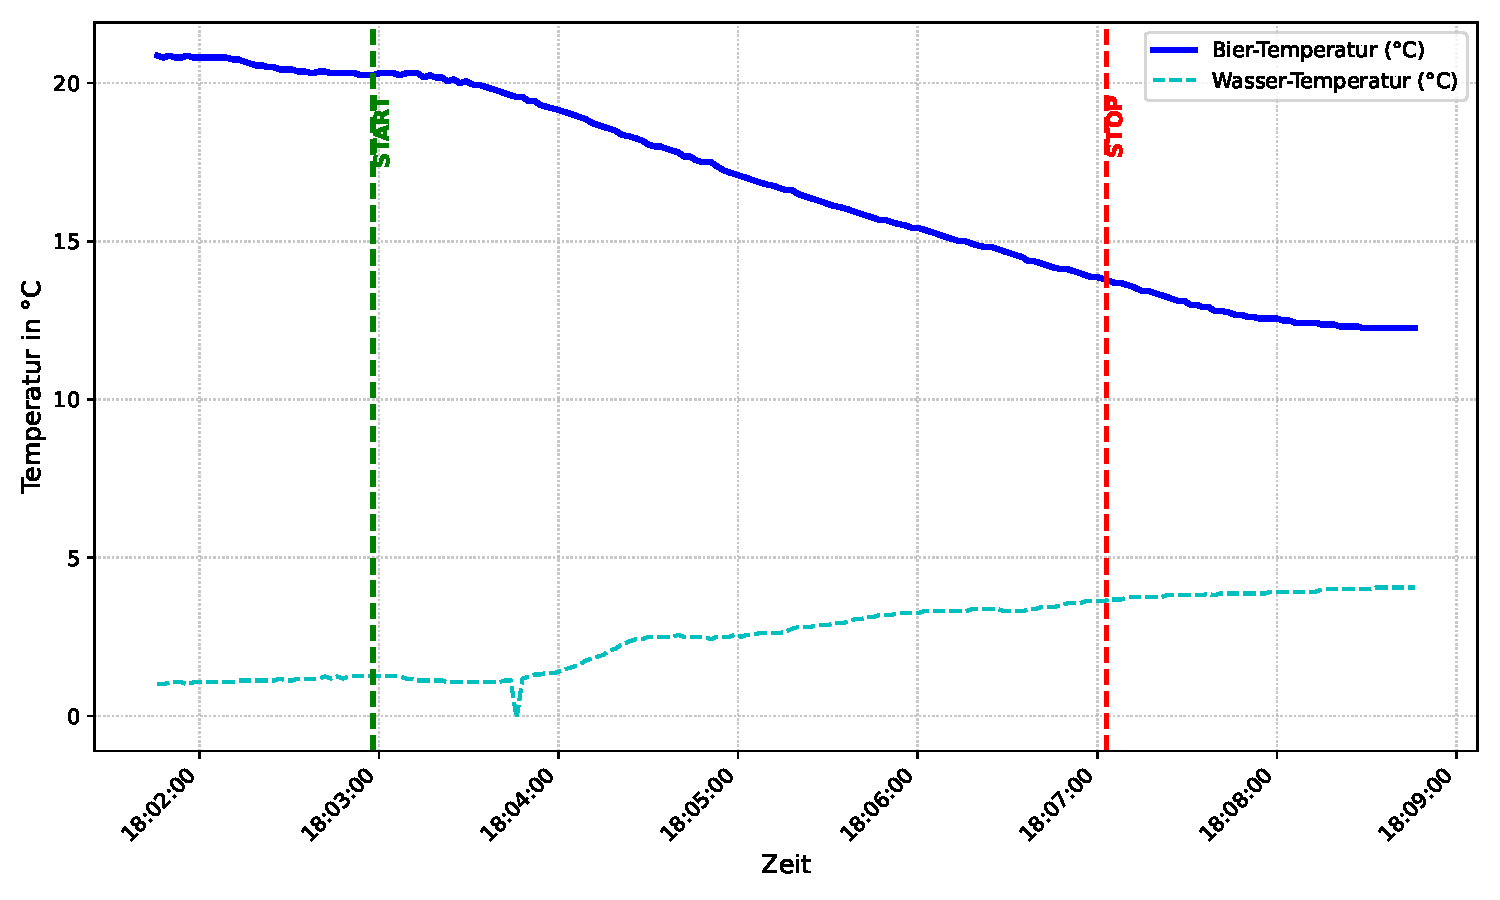
\includegraphics[width=\textwidth]{images/kuehlverlauf-bier-offen.pdf}
	\caption{Baseline-Messung mit Thermometer im offenen, zu 2/3 gefüllten Bier}
	\label{fig:baseline-messung}
\end{figure}

Zum aktuellen Zeitpunkt der Validierungsphase wurde eine erste \textit{Baseline-Messung} (Proof of Concept) durchgeführt (vgl. Abbildung~\ref{fig:baseline-messung}), um die prinzipielle Funktionalität des Kühlsystems und der Datenaufzeichnung zu verifizieren. Aufgrund der konstruktiven Neigung des Kühlbehälters wurde dieser erste Testlauf mit einer geöffneten und lediglich zu zwei Dritteln gefüllten Flasche durchgeführt, um ein Überlaufen der Flüssigkeit während der Rotation zu verhindern. Der DS18B20-Sensor zur Messung der Biertemperatur wurde dabei direkt in die Flüssigkeit innerhalb der rotierenden Flasche eingeführt. 

Diese Vorab-Messung lieferte bereits entscheidende Erkenntnisse:
\begin{enumerate}
	\item Das Python-basierte Datenlogging inklusive der Start-/Stopp-Marker via EXTI-Interrupt funktionierte lückenlos und lieferte valide CSV-Datensätze.
	\item Das Kühlkonzept (Zusammenspiel aus Eiswasser-Pumpe und Flaschenrotation) bewirkte einen messbaren und kontinuierlichen Temperaturabfall in der Testflüssigkeit.
\end{enumerate}

Nach der erfolgreichen Bestätigung dieser Kernfunktionen (TC1 bis TC3) wurde als nächster Schritt die finale Validierungsmessung mit einer vollständig geschlossenen Flasche unter realen Betriebsbedingungen angesetzt.

\section{Analyse der Systemdynamik und thermischen Trägheit}

\begin{figure}[h]
	\centering
	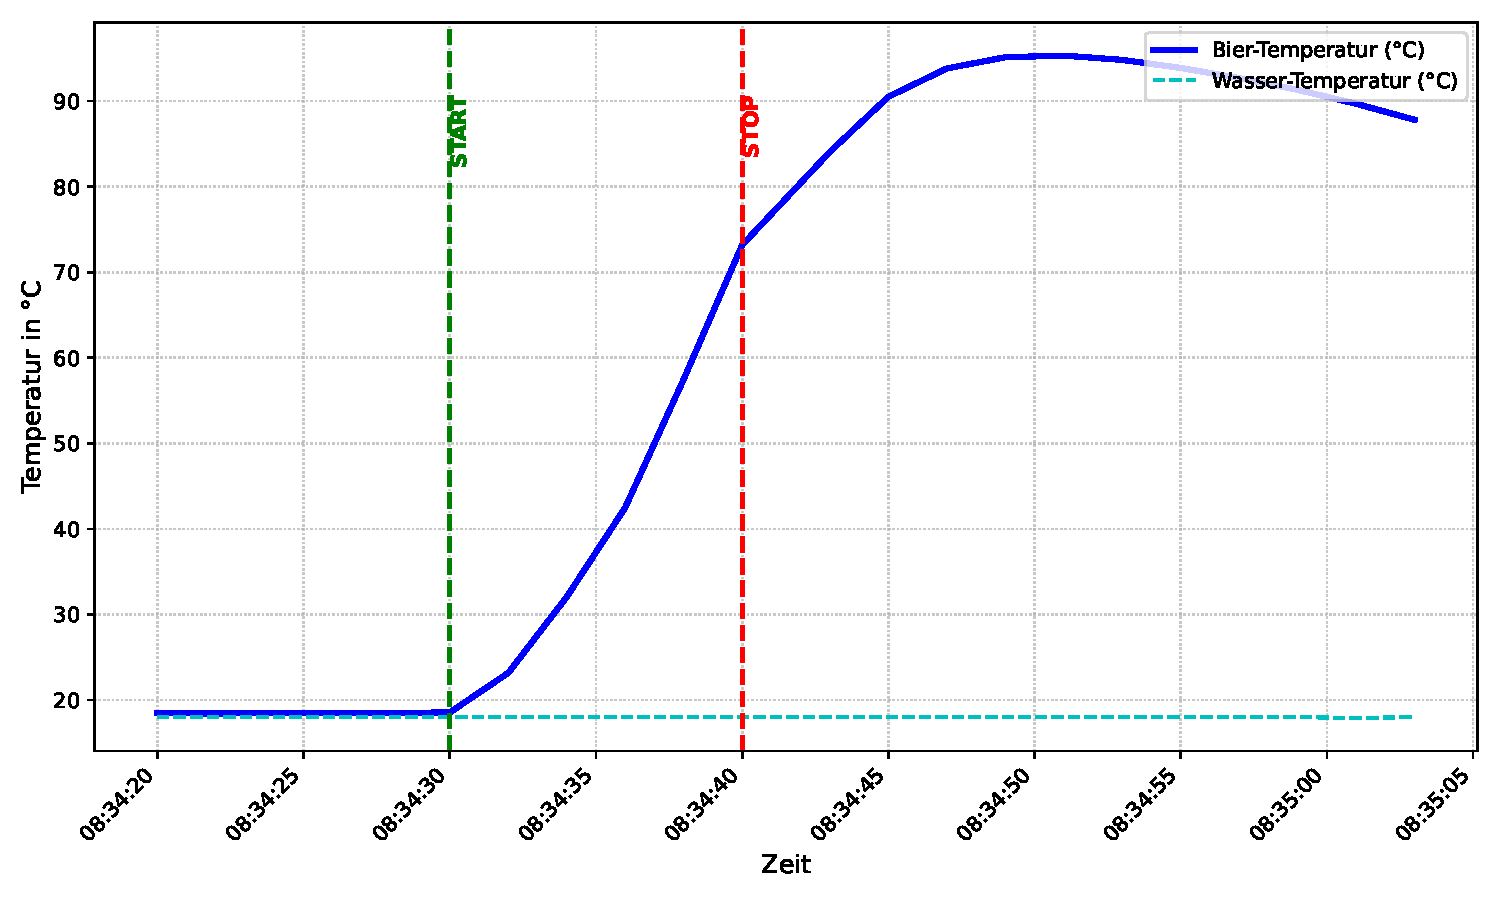
\includegraphics[width=\textwidth]{images/validierung-thermometer.pdf}
	\caption{Validierungsmessung der thermischen Trägheit des DS18B20-Sensors}
	\label{fig:validierung-thermometer}
\end{figure}

Bei der Auswertung der Baseline-Messung sowie zusätzlicher Stresstests der Sensorik fiel eine zeitliche Verzögerung in der Temperaturerfassung auf. Um dieses Verhalten quantitativ zu untersuchen, wurde eine separate Kennlinie des verwendeten DS18B20-Sensors mittels direkter Hitzeeinwirkung (offene Flamme) aufgezeichnet. Die Abbildung~\ref{fig:validierung-thermometer} zeigt die Kennlinie. Die dargestellte ,,Bier-Temperatur'' entspricht hierbei der direkten Temperatur des Thermometers über der Flamme.

Während des Tests wurde der Sensor für 10 Sekunden einer starken Wärmequelle ausgesetzt (Intervall zwischen den Markern START und STOP). Bei Beendigung der Hitzeeinwirkung (STOP-Marker) registrierte der Sensor einen Wert von etwa 73\,°C. Anstatt sofort abzukühlen, stieg die gemessene Temperatur für weitere 11 Sekunden kontinuierlich an, bis sie ihr absolutes Maximum von 95,31\,°C erreichte.

Dieser Effekt lässt sich auf die \textit{thermische Trägheit} (Wärmekapazität und Wärmewiderstand) des Sensor-Aufbaus zurückführen. Bei der verwendeten wasserdichten Variante des DS18B20 ist der eigentliche Halbleiterchip in eine Edelstahlhülse eingefasst und mit einer thermisch leitfähigen Vergussmasse isoliert. Thermische Energie benötigt eine gewisse Zeit, um diese Materialschichten zu durchdringen, was zu der gemessenen Totzeit des Systems führt.

Auch in der Baseline-Messung des Kühlwassers (vgl. Abschnitt zuvor) ist dieser Effekt sichtbar: Nach der Aktivierung der Kühlung dauert es etwa 15 Sekunden, bis der Sensor den Temperaturabfall signifikant im Datenlog abbildet. Ebenso fällt die Temperaturkennlinie nach dem Abschalten der Pumpe (STOP-Marker) zunächst noch weiter ab.

\textbf{Fazit für das Gesamtsystem:}
Für zeitkritische Regelkreise im Millisekundenbereich wäre dieser Sensor ungeeignet. Für die Anwendung in einem Getränkekühler ist diese thermische Zeitkonstante von 10 bis 15 Sekunden jedoch physikalisch vernachlässigbar. Der thermodynamische Prozess des Abkühlens einer Glasflasche mitsamt Flüssigkeit ist um ein Vielfaches langsamer als die Trägheit des Sensors, weshalb die Systemfunktion durch diesen Hardware-Effekt nicht negativ beeinträchtigt wird.

\section{Ergebnisse der Validierungsmessungen und Systemgrenzen}

\begin{figure}[h]
	\centering
	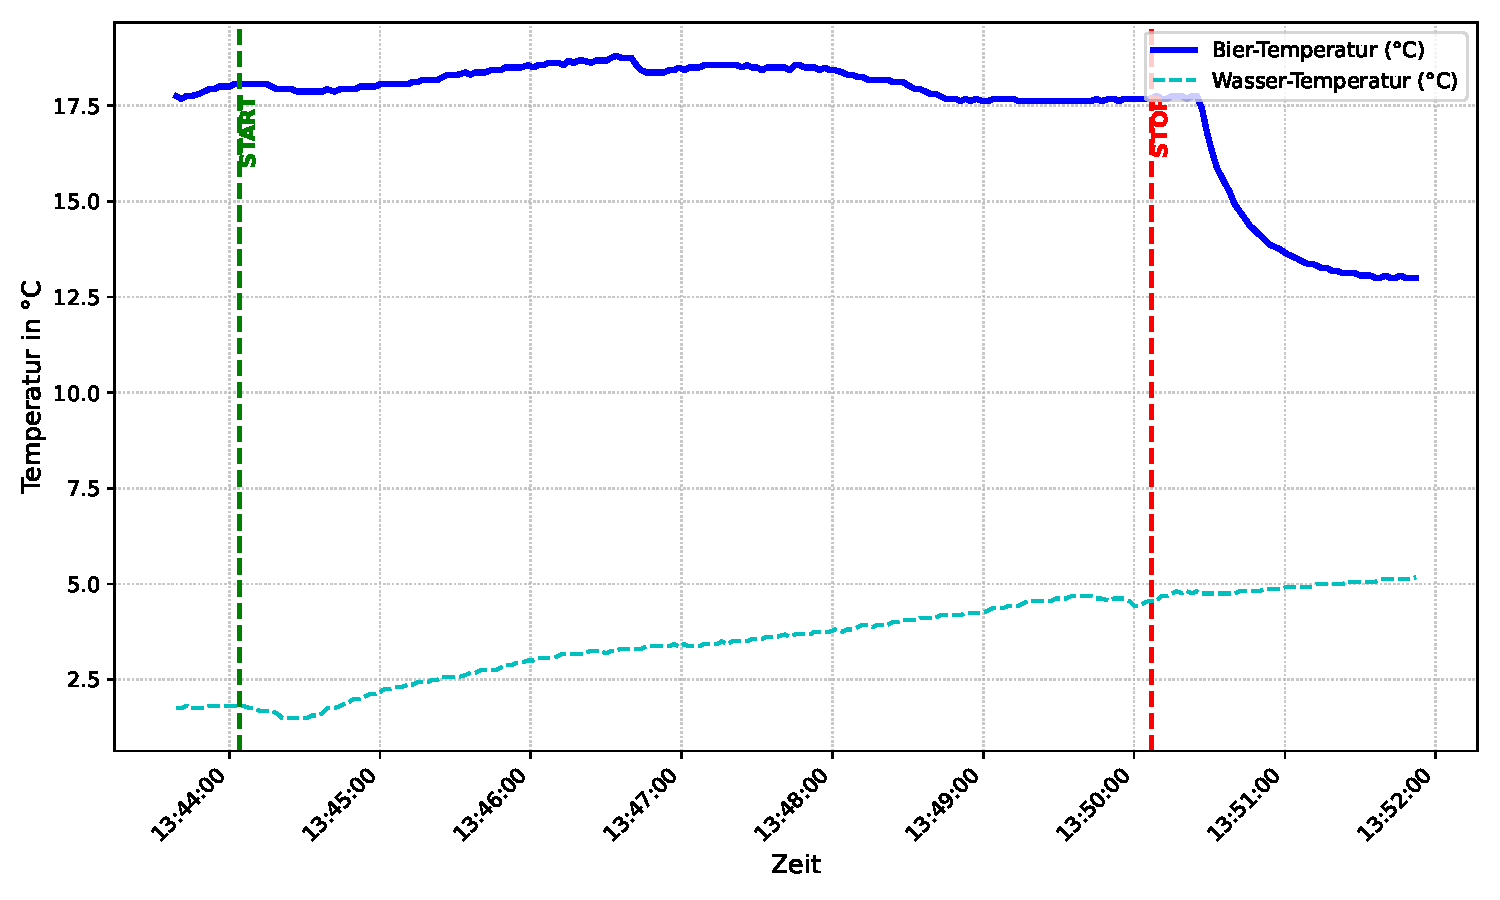
\includegraphics[width=\textwidth]{images/kuehlverlauf-bier-zu.pdf}
	\caption{Finaler Testlauf des Prototyps mit geschlossener Flasche}
	\label{fig:finaler-testlauf}
\end{figure}

Zur abschließenden Validierung des Gesamtsystems wurde ein finaler Testlauf unter realen Betriebsbedingungen mit einer vollständig geschlossenen Flasche durchgeführt (vgl. Abbildung~\ref{fig:finaler-testlauf}). Die Auswertung der protokollierten CSV-Daten brachte dabei wichtige Erkenntnisse über die thermodynamischen und mechanischen Grenzen des Prototyps zutage.

\subsection{Vergleich der Temperaturverläufe und Messmethodik}
Bei der Betrachtung der beiden Messreihen fällt ein deutlicher methodischer Unterschied auf. In der Baseline-Messung befand sich der Temperatursensor während des gesamten Rotationsvorgangs direkt in der Flüssigkeit. Dies resultierte in einer kontinuierlichen, sauberen Abkühlkurve, bei der die Temperatur über einen Zeitraum von rund 5,5 Minuten von 20,31\,°C auf 12,25\,°C gesenkt werden konnte.

Im realen Anwendungsfall (geschlossene Flasche) ist eine kontinuierliche Messung in der Flüssigkeit durch einen kabelgebundenen Sensor während der Rotation physikalisch nicht möglich. Der Sensor erfasste in diesem Zeitraum (ca. 6 Minuten Kühlzeit) lediglich die Umgebungstemperatur nahe der Flasche. Erst nach dem Stoppen der Aktorik wurde die Flasche geöffnet und der Sensor eingeführt. Dies erklärt den sprunghaften, steilen Abfall (Knick) in der Temperaturkennlinie kurz nach dem STOP-Marker. Die tatsächliche Biertemperatur fiel bei diesem Testlauf von anfänglich 18,06\,°C auf eine Endtemperatur von 13,0\,°C.

\subsection{Analyse der Kühlleistung und Eisknappheit}
Die erreichte Abkühlung um rund 5\,°C innerhalb von 6 Minuten bestätigt, dass das mechanische Kühlkonzept (Rotation im Wasserbad) grundsätzlich sehr gut funktioniert. Dennoch liegt die Endtemperatur von 13,0\,°C noch etwas über der idealen Trinktemperatur für ein kühles Bier.

Die Ursache hierfür lag an einer Eisknappheit im Wasserreservoir während dieses letzten Testlaufs. Kaltes Wasser alleine reicht nicht aus, um eine Glasflasche in so kurzer Zeit schockzukühlen. Normalerweise entzieht das schmelzende Eis dem Bier die meiste Wärme. Da in diesem Durchlauf kaum noch Eis vorhanden war, nahm das Kühlwasser die Wärme der Flasche direkt auf und erwärmte sich relativ schnell (von 1,8\,°C beim Start auf über 5,1\,°C am Ende). Je wärmer das Wasser wird, desto schlechter kühlt es die Flasche. Mit einer ausreichenden Menge an Eiswürfeln bliebe das Wasser konstant nahe dem Gefrierpunkt, wodurch sich das Bier in der gleichen Zeit noch deutlich stärker hätte abkühlen lassen.

\subsection{Mechanische Systemgrenzen und Verschleiß}
Ursprünglich war geplant, den finalen Testlauf nach der Beschaffung neuer Eisreserven mit einer längeren Rotationsdauer zu wiederholen, um die Zieltemperatur zu erreichen. Dieser Plan musste jedoch aufgrund eines kritischen Hardware-Ausfalls revidiert werden. 

Die Antriebswelle des 12V-Getriebemotors, welche die Kraftübertragung zur Flaschenrotation sicherstellt, erlitt durch die dynamischen Belastungen und das Drehmoment der vollen Flasche einen mechanischen Verschleiß (Abrieb der Passung). Dieser Verlust der formschlüssigen Kraftübertragung führte dazu, dass die Welle durchdrehte und keine Rotation mehr stattfand. Da eine Ersatzteilbeschaffung innerhalb des Projektzeitraums nicht mehr realisierbar war, wurden die Testreihen an diesem Punkt abgeschlossen.

\textbf{Fazit der Validierung:}
Die Validierungstests haben den "Proof of Concept" der elektronischen und softwareseitigen Systemarchitektur erfolgreich erbracht. Sensoren, PWM-Aktorik, Interrupt-Steuerung und das Python-Datenlogging funktionierten lückenlos und fehlerfrei. Für eine spätere Serienreife oder Version 2.0 des Kühlsystems müssen jedoch zwei Optimierungen vorgenommen werden: Ein größeres Eis-Reservoir zur Sicherstellung der thermodynamischen Kapazität sowie eine massivere mechanische Kupplung (z.B. aus gefrästem Aluminium oder Stahl) zur dauerhaften Kraftübertragung des Rotationsmotors.